\documentclass[10pt]{article}
\usepackage[letterpaper,margin=.78in]{geometry}
\usepackage{amsmath,booktabs,array,graphicx,xurl,hyperref}
\hypersetup{hidelinks,pdftitle={S27-A: Inter-Stage Activation Intervention in HStem},pdfauthor={Research execution record}}
\graphicspath{{../figures/}}
\setlength{\parskip}{4pt}
\title{S27-A: Inter-Stage Activation Intervention in HStem}
\author{Research execution record}
\date{23 November 2026}
\begin{document}\maketitle
\section{Question, Intervention, and Execution}
The question is whether three intermediate GELU activations contribute to the existing HStem design under its fixed training procedure. This stage does not search for a better classifier or finalize a submission. It builds on S26 commit \texttt{ad5443e}; scientific code, statistics and the independent B/C plans were committed as \texttt{ff79743} before any new source waveform read or scientific fit.

No-GELU (LA) reuses S21's already defined but unexecuted H3. Exactly tokenizer modules 2, 5 and 8 change from GELU to Identity. H0 and LA have identical full initial state dictionaries in every paired seed, 133,690 parameters, five BN modules, a 32-by-64 token interface and nominal convolution-path support 350. Their supported convolution/matrix count is 95.028M MACs. GELU's elementwise work is removed, so equal partial MACs do not imply equal complete FLOPs or latency. Long-Patch (LP, 138,346 parameters) is a secondary reused comparator with different grouping, BN, nonlinear depth and compute.

With a fixed frontend input and frozen BN, LA's tokenizer is affine; the complete network remains nonlinear through the shared frontend, LayerNorm and attention. Training BN depends on batch/spatial statistics. Removing activations also changes optimization, BN trajectories and learned weights; its effect cannot be reduced to an inference-only nonlinearity or a physical RF mechanism.

Six new fits use the original two folds, seeds 201/202/203, 8,000 train and 2,000 source-validation packets per fold, 200 epochs, batch 64, AdamW, five-epoch warmup/cosine scheduling and fixed independent order/AWGN generators. Clean source RX-equal CE selects each checkpoint. All six checkpoint/configuration/history hashes were sealed and committed before common report-only target inference. H0/LP weights are reused; no new Confirm or old-blind packet is read.

\section{Complete Quantitative Result}
\begin{center}\small
\begin{tabular}{lrrrrrr}\toprule
Arm&Params&Dev acc.&Fit SD&Macro-F1&Worst RX&Source acc.\\\midrule
H0&133,690&97.335&0.552&97.326&93.667&98.175\\
LA&133,690&96.583&0.779&96.554&90.383&97.742\\
LP&138,346&94.500&1.831&94.423&88.333&96.358\\
\bottomrule\end{tabular}\end{center}
Accuracy/F1 are percentages, fit SD is in percentage points (pp) over six fold/seed means, and worst RX is the minimum three-seed RX mean. The selected source validation packets have already influenced checkpoint choice.
The primary H0--LA contrast is +0.752 pp, conditional RX 95\% interval [0.212, 1.438], with 5/6 positive paired fit means. The two fold means are +0.963 and +0.540 pp.
The registered consistency rule is met. Retaining the three GELUs benefits this complete architecture/training procedure.
LA still exceeds LP by +2.083 pp after the three GELUs are removed. These activations therefore do not account for the entire H0--LP difference. The telescoping accuracy differences are not causal contribution percentages; grouping, normalization, factorization and optimization remain confounded. The fold 0 / seed 201 H0--LA contrast is -0.200 pp; RTL-5 favors LA by0.417 pp and RTL-2 is tied. All are retained.
The rule requires a mean gain of at least 0.5 pp, a positive conditional lower bound, at least five positive fit pairs and positive means in both folds. Three seed differences are first averaged within each of ten unique RXs, then RX identities are resampled 10,000 times with seed 27027. These intervals omit fresh-seed, acquisition and architecture-selection uncertainty. They are developmental conditional summaries, not confirmatory population guarantees; no multiplicity-adjusted claim is made.
\begin{figure}[htbp]\centering
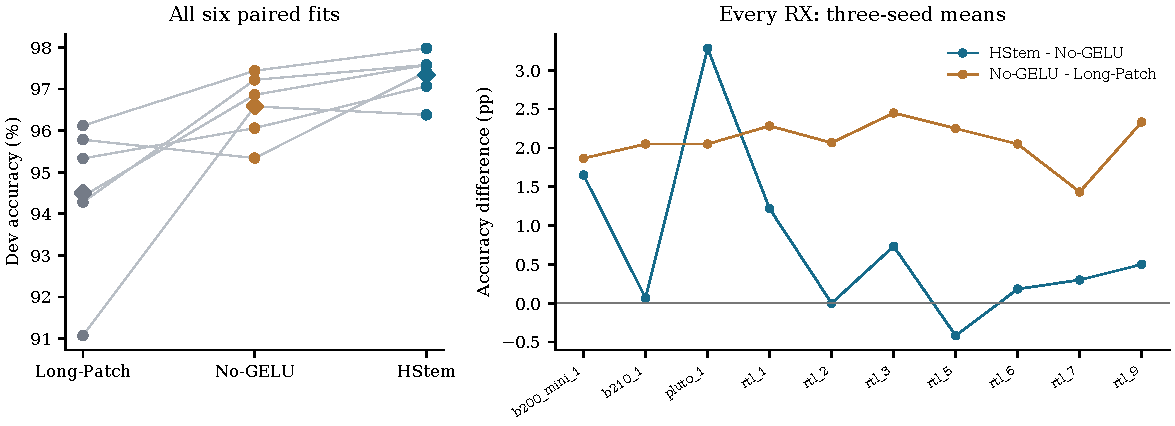
\includegraphics[width=.98\linewidth]{fig01_complete_comparison.pdf}
\caption{All six paired fits and every held RX. No seed or unfavorable receiver is removed.}
\end{figure}

\section{Source Learning and Historical Receiver Transfer}
Define $G=\operatorname{Acc}_{SourceVal}-\operatorname{Acc}_{Dev}$. Report the two accuracies alongside the difference; a smaller gap alone is not evidence of better held identification.
H0--LA source change is +0.433 pp, Dev change +0.752 pp, and $G_{H0}-G_{LA}$ is -0.318 pp. Source mean CE is 0.059022 (H0), 0.076934 (LA), and 0.107024 (LP).
Only 3/6 paired gap differences are negative, so the mean does not establish stable gap contraction.
Source validation has 40 selected packets per TX/RX, compared with 200 for Dev, and was used for selection. Every current RX also has a research history and is source in the reverse fold. Therefore this difference cannot replace the independently fitted four-source/one-held C Pilot or establish a receiver-specific suppression mechanism. Accuracy ceilings and source-fitting changes remain relevant.
\begin{figure}[htbp]\centering
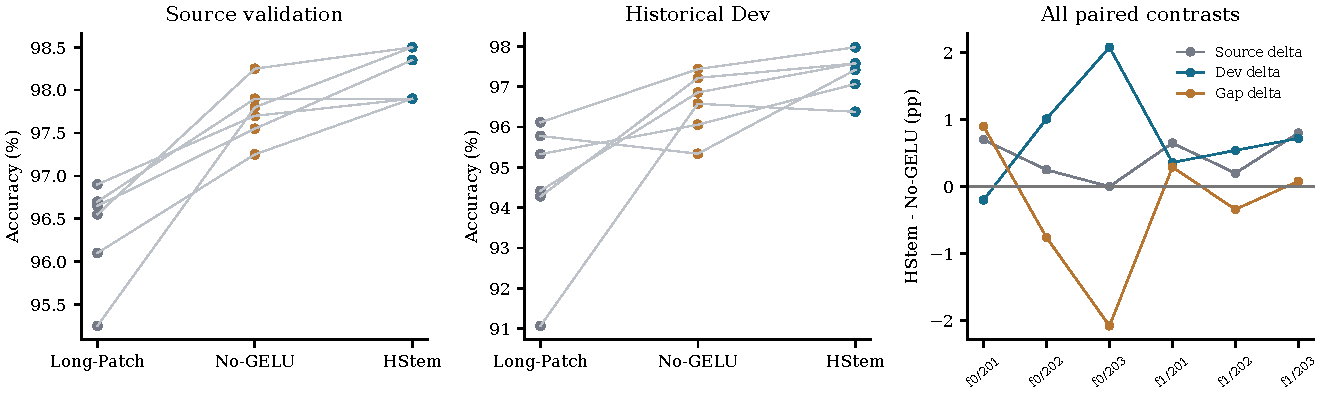
\includegraphics[width=.99\linewidth]{fig02_source_dev.pdf}
\caption{Source and Dev accuracy for every fit, and complete paired source/Dev/gap contrasts. Gap contrasts are descriptive.}
\end{figure}

\section{Every New Fit and Its Cost}
\begin{center}\small
\begin{tabular}{rrrrrrr}\toprule
Fold&Seed&Best epoch&Source CE&Source acc.&Dev acc.&Fit wall(s)\\\midrule
0&201&191&0.077271&97.800&96.580&1941.3\\
0&202&188&0.071545&98.250&96.060&1943.9\\
0&203&191&0.072020&97.900&95.340&1342.8\\
1&201&176&0.084368&97.250&97.220&1280.3\\
1&202&164&0.079308&97.700&97.440&1891.5\\
1&203&152&0.077091&97.550&96.860&1894.8\\
\bottomrule\end{tabular}\end{center}
Every new fit completes 200 epochs and 25,000 updates. Checkpoint selection uses only source CE. No seed is restarted or replaced based on scores. Summed fit wall times overlap under at most two CUDA jobs and are not exclusive GPU hours.
\begin{figure}[htbp]\centering
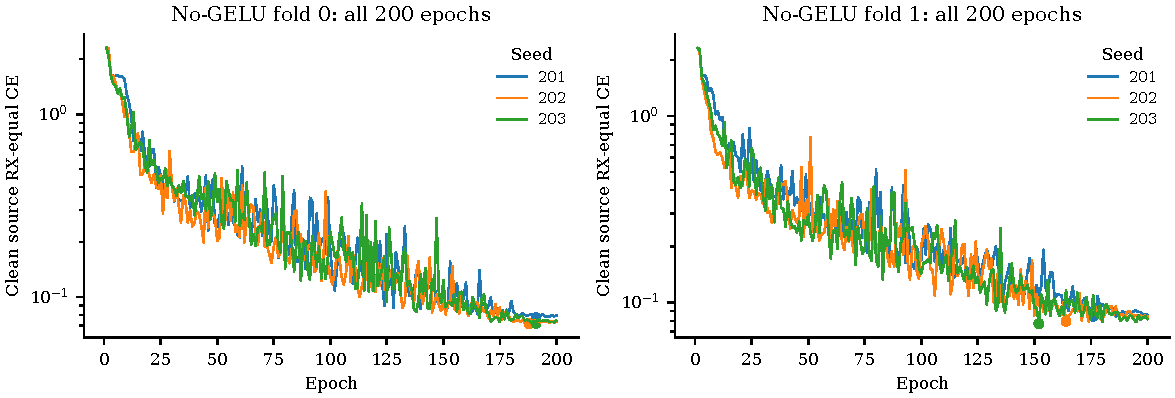
\includegraphics[width=.98\linewidth]{fig03_complete_training.pdf}
\caption{Complete source CE histories; markers show the source-selected checkpoint. Curves retain all epochs and seeds.}
\end{figure}
\begin{center}\small
\begin{tabular}{lrrr}\toprule
Arm&Partial MACs(M)&B1 p50(ms)&B128 p50(ms)\\\midrule
H0&95.028&3.216&17.370\\
LP&55.477&2.389&17.293\\
LA&95.028&2.989&16.844\\
\bottomrule\end{tabular}\end{center}
Costs use one separate GPU-resident IQ-to-logits session, FP32 tensors with matmul TF32 off and cuDNN TF32 on, three warmups and 15 repetitions. B128 is whole-batch latency, not per-packet latency. Partial MAC counts omit FFT and unsupported dispatcher operations. Measured latency includes the complete model frontend, including FFT, and excludes host transfer. No old timing session is pooled with this one.

\section{What the Intervention Identifies and Leaves Open}
The direct A contrast excludes changed parameter counts, nominal support, token geometry, initial weights, backend architecture or packet budget as explanations. It measures the effect of retaining these activations within the prescribed training procedure. It does not isolate nonlinear expressivity from optimization or BN dynamics. Layerwise geometry ratios are not mutual information or hardware invariance; no further representation tap, normalization or projection is selected from target scores.

S26's long-projection result restricts one selected support-only explanation; it does not exclude every possible long-kernel design. Neither study establishes pure hierarchy causality, antialiasing, synchronization robustness, fresh acquisition generalization, unknown-device rejection or active-attack authentication. Previous weak seeds, unfavorable RXs and severe circular-shift failures remain in the historical evidence.

\section{Frozen Next Experiments: Not Executed}
\textbf{B (planned 12 fits, executed 0).} Cross H0/LP tokenizers with original MHA and a fixed positionwise two-block residual MLP, followed by the unchanged final LN/mean/classifier. Each MLP block has 16,704 parameters versus 16,768 for MHA; whole-model counts differ by 128. Hidden width 128 follows nearest integer parameter matching without RF data. Surviving modules preserve corresponding initial states; new heads share a fixed CPU RNG stream. There is no cross-token interaction before pooling, but nonlinear depth and compute also differ. The primary contrast is
\[
(A_{H,M}-A_{LP,M})-(A_{H,P}-A_{LP,P}).
\]
It identifies relative accuracy interaction for these backends, not a universal need for attention or how RF information is encoded. Full rules and conditional RX statistics are frozen in \texttt{PLAN\_B.json}.

\textbf{C (planned 12 fits, executed 0).} A receiver-name SHA256 rule fixed b210\_1 (fold 0) and rtl\_5 (fold 1) before A evaluation. Train fresh H0/LP on the other four legal source RXs with 6,400 training / 1,600 validation packets, 200 epochs and 100 updates per epoch. The held RX contributes no optimizer, BN, scheduler or selection information; evaluate all 2,000 held packets only after a complete 12-model seal. Report held accuracy and source/held gap jointly. Only two held RX units are available; seeds do not create six independent receivers, so no population RX bootstrap is claimed. Fixed all-layer feature diagnostics use 40 last selected packets/TX/RX. Held-only across-RX centroid ratio is NA because there is one held RX; source and combined centroid/scatter diagnostics have explicitly stated domains. No score-driven receiver substitution or automatic expansion is allowed.
The current highest-value follow-up is B, as a research-priority judgment after disclosing A, with both designs unchanged. The fixed factorial backend comparison directly tests whether the tokenizer benefit depends on this MHA readout. Neither experiment is launched in this stage. IQ-only, ASK Strict-IB and any extra architecture/seed search also remain unexecuted.

\section{Integrity and Reproduction}
Independent recomputation checks 180,000 saved packet predictions across 90 model/RX cells, balanced labels and row identities, confusion matrices, accuracy, macro-F1, conditional paired intervals, source selection, first permutation/AWGN streams and historical checkpoint/config/history hashes. CE is independently derived from saved logits; the original evaluator does not archive a target CE field. Source recovery and common baseline-logit recovery are reported explicitly, without overwriting historical results.

The gate checks active-source syntax/imports, capacity, exact initial states, forbidden roles, finite gradients, batch 64/128 resources and exact optimizer/RNG resumed updates. An initial JSON-serialization variable collision was corrected before preregistration; eight synthetic updates in total are separately recorded, not counted as scientific fits. A later Windows file-sharing error interrupted a progress-file atomic rename after the epoch 6 snapshot (750 updates) was saved. A separately registered IO-only retry wrapper retained all frozen scientific bytes and restored the model, optimizer and complete RNG state at epoch 7. Thus six independent fits used seven training-process invocations without repeating completed updates. Original failures and recovery hashes are retained. All six new fits complete 150,000 scientific optimizer updates. No failure or unfavorable seed is deleted.

\href{https://github.com/hanCChan/crossatten/tree/exp/s27-mechanism-identification/27-mechanism-identification}{Repository evidence, code, real logs and Chinese research report} accompanies this record. Large waveforms, checkpoints, resume states and sample-level predictions remain local. Aggregate figures/documents can be rebuilt from the committed JSON/CSV evidence, without refitting or reading RF data. This stage supplies mechanism evidence; it does not certify novelty or submission readiness.
\end{document}
